\documentclass[titlepage, 13px, a4paper]{report}

\usepackage[utf8]{inputenc}

\usepackage[T1]{fontenc}
\usepackage{fontawesome}
\usepackage{eurosym}

\usepackage[french]{babel}

\usepackage{fancyhdr}
\usepackage{graphicx}
\usepackage[left=4.5cm,right=4cm,top=4.5cm, textheight=17cm]{geometry}
\usepackage{wrapfig}

\usepackage{eso-pic}
\usepackage{transparent}

\usepackage{hyperref}
\usepackage{setspace}

\usepackage{titletoc}
\usepackage{titlesec}

\usepackage{stackengine,xcolor}
\usepackage{enumerate}

\titleclass{\part}{top}
\titleformat{\part}[display]
  {\normalfont\huge\bfseries}{\centering\partname\ \thepart}{20pt}{\Huge\centering}
\titlespacing*{\part}{0pt}{50pt}{40pt}
\titleclass{\chapter}{straight}
\titleformat{\chapter}[display]
  {\normalfont\huge\bfseries}{\chaptertitlename\ \thechapter}{20pt}{\Huge}
\titlespacing*{\chapter} {0pt}{50pt}{40pt}

%\usepackage{titlesec}
%\titleformat{\part}[display]
  %{\normalfont\bfseries}{}{0pt}{\Large\bfseries}

\newcommand\BackgroundPic{%
	\put(0,-50){%
		\parbox[b][\paperheight]{\paperwidth}{%
			%\vfill
			\centering
			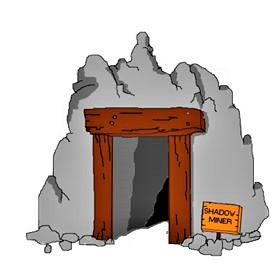
\includegraphics[%
			keepaspectratio]{../images/icone.jpg}%
			\vfill
		}
	}
}

\fboxrule=2pt
\newcommand\cincludegraphics[2][]{%
  \setbox0=\hbox{\includegraphics[#1]{#2}}%
  \abovebaseline[-.5\ht0]{\includegraphics[#1]{#2}}}

  
\renewcommand{\baselinestretch}{1}
\renewcommand{\partname}{}


\title{\textbf{{\Huge Manuel d'utilisation}}}
\author{
	\\
	\bsc{{\LARGE \bf ShadowMiner}} \\ \\ \\
	\bsc{{\LARGE \bf par ACCEr}} \\ \\
}
\date{{\LARGE \today}}

\pagestyle{fancy}
%\fancyfoot[L]{
\includegraphics{../images/ShadowMiners_logo_mini.png}} %50x33
\fancyfoot[L]{\cincludegraphics[scale=0.1]{../images/ShadowMiners_logo.png}} %50x33
\fancyfoot[R]{STRASBOURG 2022}
\fancyhead[R]{ACCEr}
\fancyhead[L]{Manuel d'utilisation}

\setcounter{tocdepth}{3}

\begin{document}
\AddToShipoutPicture*{\BackgroundPic}

\maketitle
\tableofcontents
%\listoftables
%\listoffigures

%################### INTRO

\fancypagestyle{plain}{}
\stepcounter{chapter}
\part{Introduction} 
\paragraph{} \hspace{0pt}
r

%################### INTRO


\newpage

%################### Qui sommes nous ?

\fancypagestyle{plain}{}
\stepcounter{chapter}
\part{Qui sommes nous ?}
\section{Présentation des membres du groupe}

\paragraph{~~~~Cédric} \hspace{0pt}

\paragraph{~~~~Antoine} \hspace{0pt}

\paragraph{~~~~Clément} \hspace{0pt}

\paragraph{~~~~Edgar} \hspace{0pt}


\section{L'origine du nom du groupe : \textit{ACCEr}}
\paragraph{} \hspace{0pt}
Le nom du groupe provient d’Antoine. A l’origine, nous nous appelions ACCer avant l’arrivée d’Edgar. 
« ACC » pour les initiales de nos prénoms et « er » pour porter confusion entre notre groupe 
et la société taïwanais ACER, constructeur informatique. \\ \\
A l’arrivée d’Edgar, on a décidé de mettre en majuscule le « e » de notre nom. \\
C’est ainsi qu’ACCEr est né.

\newpage

\section{Planning}
\paragraph{} \hspace{0pt}
Voici un rappel de notre planning annoncé dans le cahier des charges :
\\ \\
{\small
	\begin{tabular}{|p{7.2cm}|p{1.2cm}|p{1.2cm}|p{1.2cm}|}
		\hline
		Pourcentages des tâches & \multicolumn{3}{|c|}{jusqu'à la soutenance} \\ 
		\cline{2-4}
			& \no 1 & \no 2 & \no 3 \\
		\hline
		Création des préfabs de map pour les niveaux (murs, sol, porte, ..) & 75\% & 100\% & 100\% \\
		\hline
		Modélisation 3D pour de meilleurs graphismes (si possible) & 0\% & 75\% & 100\% \\
		\hline
		Script c\# animation & 30\% & 60\% & 100\% \\
		\hline
		Création des préfabs des joueurs & 100\% & 100\% & 100\% \\
		\hline
		Script c\# joueur & 50\% & 75\% & 100\% \\
		\hline
		Création de multiples niveaux (entre 20 et 40) & 10-20\% & 50\% & 100\% \\
		\hline
		Création du Shadow Miner et Script c\# pour l'IA du Shadow Miner & 30\% & 60\% & 100\% \\
		\hline
		Cinématique du jeu & 0\% & 50\% & 100\% \\
		\hline
		Son du jeu & 0\% & 30\% & 100\% \\
		\hline
		Menu du jeu & 0\% & 40\% & 100\% \\
		\hline
		Création du site internet et Hébergement en ligne & 40\% & 80\% & 100\% \\
		\hline
		Création du serveur multijoueurs & 40\% & 90\% & 100\% \\
		\hline
		Création des joueurs pour multijoueurs & 30\% & 90\% & 100\% \\
		\hline
		Création du système de map aléatoire pour le multijoueurs & 0\% & 20\% & 100\% \\
		\hline
		Compilation du jeu et enregistrement sur CD & 0\% & 0\% & 100\% \\
		\hline 
		\end{tabular}
	\label{Planning}	
}


%################### Qui sommes nous ?


\newpage

%################### ShadowMiner

\fancypagestyle{plain}{}
\stepcounter{chapter}
\part{Le jeu : ShadowMiner}
\section{Le mode solo}

\subsection[Scénario]{~~~~Scénario}
\paragraph{} \hspace{0pt}
\begin{quotation}
	Un mineur descend tôt le matin dans les derniers sous-sols de la mine, là où l’oxygène se fait rare. 
	Un mineur fou (le Shadow Miner) coupe les câbles de l’ascenseur. 
	Le mineur veut alors rejoindre la surface. Le Shadow Miner va alors vouloir l’en empêcher. \\
\end{quotation}

\subsection[Gameplay]{~~~~Gameplay}
\paragraph{} \hspace{0pt} \\
L’utilisateur incarne alors le mineur. \\
Le joueur devra donc progresser dans une série de niveaux de plus en plus difficiles. \\
Des pièges tels que des piques ou des traps seront là pour le ralentir. \\
Le ShadowMiner lui-même sera là pour le traquer et le capturer dans les niveaux les plus difficiles. \\
Chaque niveau symbolise un étage de la mine. Le joueur devra donc rejoindre un checkpoint 
qui symbolise la fin d’un niveau pour passer à l’étage suivant et donc au niveau suivant. \\
Le dernier niveau est donc la sortie de la mine. \\ 

\subsection[Progression du joueur]{~~~~Progression du joueur}
\paragraph{} \hspace{0pt} \\
Le joueur devra réussir le niveau actuel pour accéder au niveau suivant. \\ \\
La progression du joueur est visible en jeu et sur le site internet \url{https://accer.ddns.net} si le joueur a liée son compte au jeu. \\

\newpage

\section{Le mode multijoueurs}

\subsection[Prérequis]{~~~~Prérequis}
\paragraph{} \hspace{0pt} \\
Le joueur devra créer un compte pour pouvoir accéder au mode multijoueurs. \\
Ce compte pourra être créer sur le site internet \url{https://accer.ddns.net} ou dans le jeu lui-même Ainsi le joueur pourra 
consulter et modifier ses données depuis le site internet \url{https://accer.ddns.net} ou depuis le jeu. Ce système lui permet 
de jouer sur n’importe quel exécutable du jeu en conservant ses données. 
Cela accroit fortement la portabilité du jeu. \\

\subsection[Gameplay]{~~~~Gameplay}
\paragraph{} \hspace{0pt} \\
Le joueur rejoint tous d’abord un lobby où il doit attendre que trois joueurs 
soient connectés avant que la partie ne commence.

\paragraph{} \hspace{0pt} \\
Un joueur incarnera le ShadowMiner et devra tuer les deux autres joueurs qui 
incarneront deux mineurs voulant rejoindre la surface. Un des mineurs pourra 
s’enlever la vie et devenir un esprit de la mine qui contrôle les cloisons de 
la mine (porte, mur, gouffre) pour aider l’autre mineur. \\

\paragraph{~~~~Comment gagner ?} \hspace{0pt}
{\begin{itemize}
	\item Le ShadowMiner doit tuer tous les mineurs pour remporter la partie,
	\item Les mineurs doivent survivre jusqu’à la fin du minuteur pour remporter la partie. \\
\end{itemize}}

\subsection[Score du joueur]{~~~~Score du joueur}
\paragraph{} \hspace{0pt} \\
Le joueur gagnera en score à chaque victoire en mode multijoueurs. \\
Son score sera visible en jeu mais aussi sur le site internet \url{https://accer.ddns.net}. \\
Un classement des meilleurs joueurs est d’ailleurs disponible sur le site internet \url{https://accer.ddns.net}. \\


\newpage

\section{Le site web}
\paragraph{} \hspace{0pt}
a

\section{Technologies utilisées}
\paragraph{} \hspace{0pt}
a

%################### ShadowMiner

\newpage

%################### Réalisation individuelle

\fancypagestyle{plain}{}
\stepcounter{chapter}
\part{Réalisation individuelle}
\section*{Contexte}
\paragraph{} \hspace{0pt}
r

\newpage
\section{Antoine}
\paragraph{} \hspace{0pt}
r

\newpage
\section{Cédric}
\paragraph{} \hspace{0pt}
r

\newpage
\section{Clément}
\paragraph{} \hspace{0pt}
r

\newpage
\section{Edgar}
\paragraph{} \hspace{0pt}
r

\newpage
\section{Conclusion}
\paragraph{} \hspace{0pt}
r

%################### Réalisation individuelle

\newpage

%################### Sources et remerciements

\fancypagestyle{plain}{}
\stepcounter{chapter}
\part{Sources et remerciements}
\paragraph{} \hspace{0pt}
r

%################### Sources et remerciements

\newpage

%################### Quelques images du jeu

\fancypagestyle{plain}{}
\stepcounter{chapter}
\part{Quelques images du jeu}


%################### Quelques images du jeu

\newpage

%################### Conclusion

\fancypagestyle{plain}{}
\stepcounter{chapter}
\part{Conclusion}
\paragraph{} \hspace{0pt}
Conclusion

%################### Conclusion

\newpage

%################### Glossaire

\fancypagestyle{plain}{}
\stepcounter{chapter}
\part{Glossaire}
\paragraph{} \hspace{0pt}
G

%################### Glossaire

\end{document}